\clearpage
\pagenumbering{arabic}
\setcounter{page}{1}

\phantomsection
\label{ch:intro}
\chapter{Introduction}

This chapter presents about what is OCR? why it is needed, and
what are the challenges in OCR. It also presents the problem 
for OCR on Khmer script (non-latin based), and OCR on multilingual
language such as Khmer and English. We will talk about the scope
of this research because it'll help us to keep 
our research scope ensures clarity, direction, and feasibility 
throughout the study.

\section{Background to the Study}
\label{sec:background}

Optical Character Recognition (OCR) has changed how we turn printed text into digital formats. Thanks to AI advances, OCR systems now use deep learning to detect and classify characters from images. This technology powers digital libraries, search systems, and language processing tools.

OCR works great for major languages like English, Chinese, and Japanese. These languages have tons of training data and well-studied text structures. But OCR for smaller languages like Khmer? That's a different story.

Cambodia needs OCR technology more than ever. Over the past 20 years, the country has gone digital fast. People want to digitize Khmer documents for education, research, and everyday use. But here's the problem: Khmer script is incredibly complex.

Khmer writing goes back to the 7th century. It's not like English where letters sit in a row. Khmer characters stack on top of each other. They have subscripts, diacritics, and vowel markers that can appear above, below, or around the main character. Miss one tiny mark and you change the whole meaning of a word.

\begin{table}[ht]
    \caption{Why Khmer OCR is Desperately Needed}
    \vspace{10pt}
    \phantomsection
    \label{sec:textbook}
    \resizebox{\textwidth}{!}{
    \begin{tabular}{|l|l|l|}
    \hline
    Sector & Current Problem & Impact \\
    \hline
    Education & Physical textbooks only & Students can't search or edit content \\
    Libraries & Books rotting on shelves & Knowledge becomes inaccessible \\
    Government & Paper records everywhere & Slow bureaucracy, hard to find documents \\
    Healthcare & Handwritten patient files & Doctors waste time, medical errors increase \\
    Business & Manual data entry & Companies lose money on inefficiency \\
    Culture & Ancient texts deteriorating & We're losing our heritage \\
    \hline
    \end{tabular}
    }
\end{table}

Look at education. Most school textbooks exist only on paper. The original digital files? Gone. Lost. This creates real problems for students who need accessible learning materials.

But it's bigger than just schools. Ancient palm leaf manuscripts are crumbling. Government documents pile up in storage rooms. Hospitals still use paper files that doctors can't read properly. Businesses waste hours typing data that OCR could handle in minutes.

And here's what's really frustrating: while Google can read English text perfectly, it struggles with basic Khmer sentences. The technology gap is huge.

The thing is, Khmer OCR isn't just a nice to have anymore. It's essential for Cambodia's digital future. The country needs this technology to preserve its culture, modernize its institutions, and give its people better access to information.

That's exactly why this research matters. We're not just building another OCR system. We're creating technology that could unlock thousands of years of Khmer knowledge and make it searchable, editable, and accessible to everyone.


\section{Problem Statement}
\label{sec:problem}

Optical Character Recognition (OCR) for the Khmer language presents a 
unique set of challenges that significantly hinder the development 
of accurate and robust recognition systems. Unlike Latin-based scripts, 
Khmer is an abugida writing system, where each character represents a 
consonant-vowel unit and includes complex combinations of base 
characters, subscripts, superscripts, and diacritics. This structural 
complexity introduces difficulties at both the text detection 
stage and the text recognition stage.
\begin{figure}[ht]
    \centering
    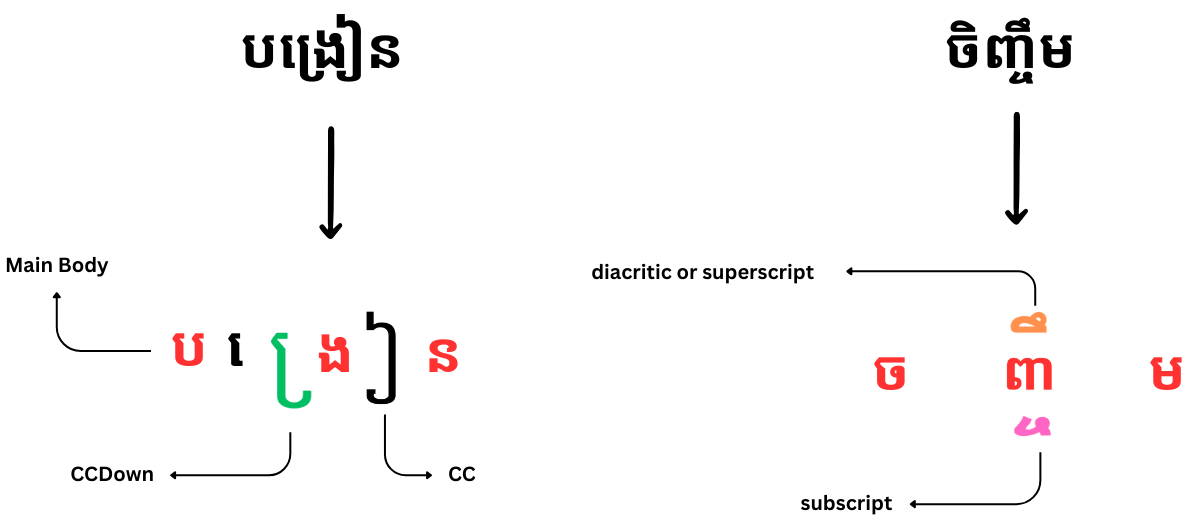
\includegraphics[width=\textwidth]{figures/example_of_text_format.png}
    \caption{Example of Khmer text format showing the complexity of character combinations and diacritics}
    \label{fig:text_format}
\end{figure}

One of the fundamental obstacles is the lack of clear word boundaries 
in Khmer writing. In contrast to Latin-based languages, 
where spaces are consistently used to separate words, 
spaces in Khmer are used infrequently and inconsistently. 
This makes it extremely difficult to segment text accurately 
into word-level units for training sequence-to-sequence OCR models 
such as TrOCR. The absence of reliable word boundaries reduces 
recognition accuracy and complicates tasks like error correction, 
search indexing, and language modeling.

\begin{figure}[ht]
    \centering
    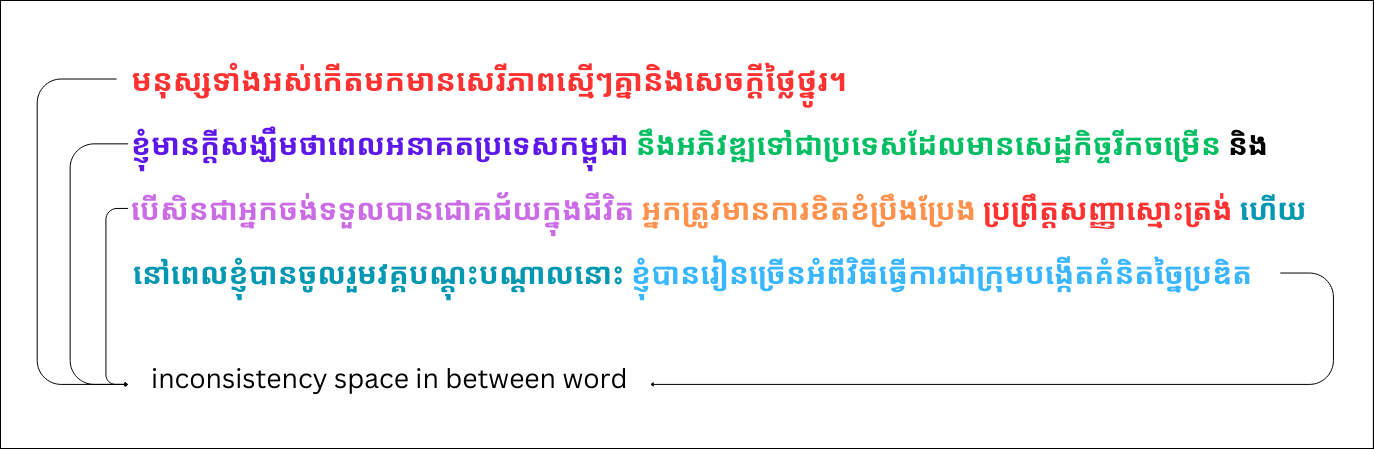
\includegraphics[width=\textwidth]{figures/example_of_long_text.png}
    \caption{Example of sequential Khmer text showing how characters combine to form syllables and words}
    \label{fig:sequential_text}
\end{figure}


A critical barrier to advancing Khmer OCR is the scarcity of annotated training datasets. There is a severe lack of high-quality, large-scale datasets that provide paired image-text data with bounding boxes, character-level annotations, or transcription lines tailored to Khmer script. This data scarcity limits the potential for supervised learning approaches and transfer learning, which are essential for training modern deep OCR models like TrOCR.


Additionally, font and style variability further degrade recognition performance. Khmer documents in the real world are printed in diverse typefaces and stylistic variations (e.g., Khmer OS, Nokora, and Hanuman), with differences in stroke thickness, spacing, and decoration. The lack of standardization across documents and poor documentation of these fonts means that OCR models trained on one style often fail to generalize to others. This problem is exacerbated in noisy or low-resolution scans of textbooks and historical texts.

The challenge of font variability is illustrated in Figure \ref{fig:font_variants}, which shows how the same Khmer text can appear significantly different across various fonts and styles.

\begin{figure}[ht]
    \centering
    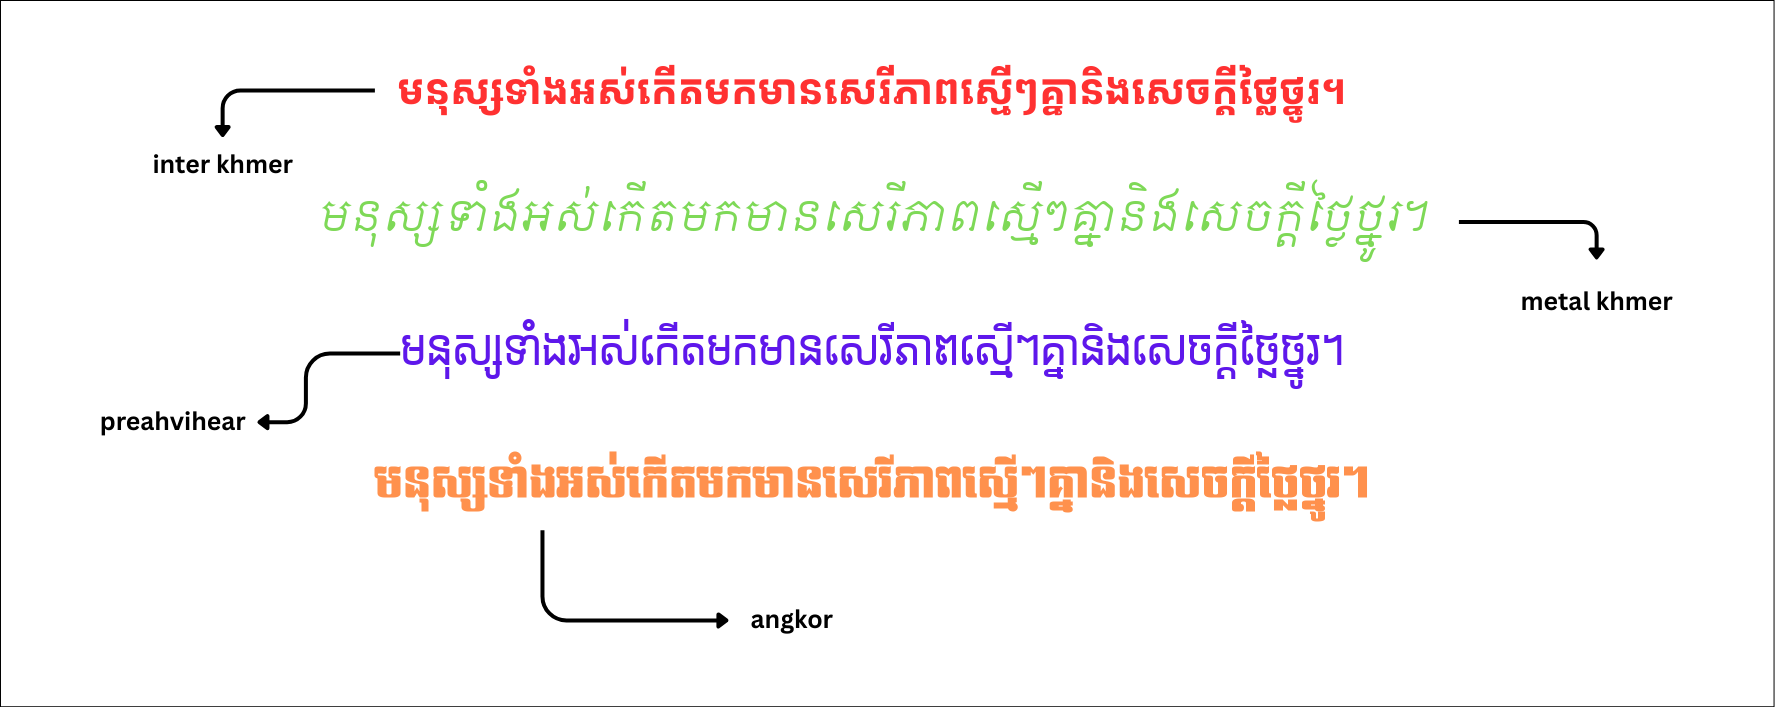
\includegraphics[width=\textwidth]{figures/varianty_of_font.png}
    \caption{Examples of the same Khmer text rendered in different fonts, demonstrating the significant visual variations that OCR systems must handle}
    \label{fig:font_variants}
\end{figure}

\begin{figure}[ht]
    \centering
    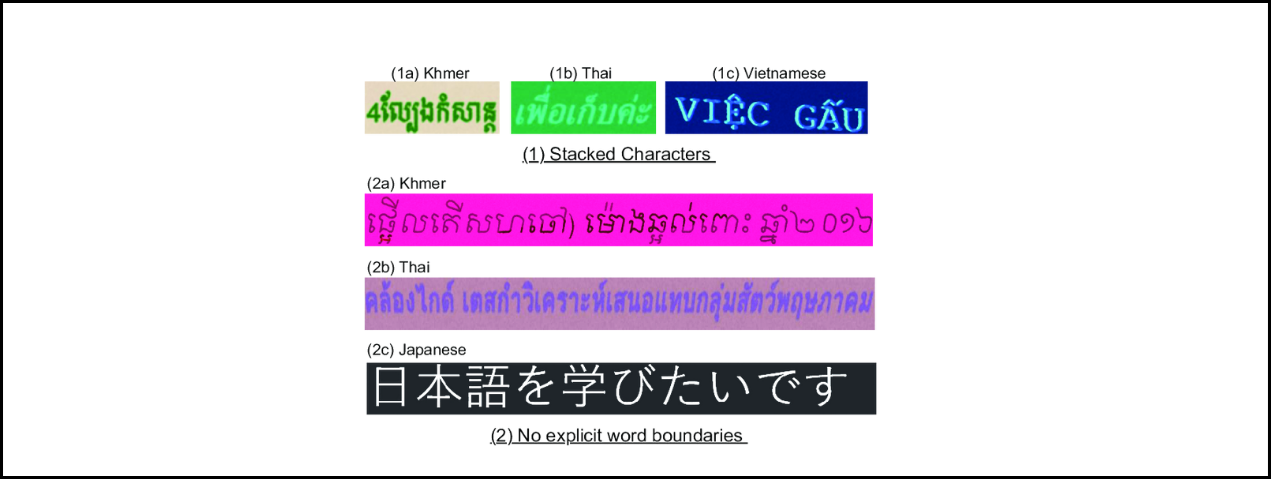
\includegraphics[width=\textwidth]{figures/text_stacking_mixing_language.png}
    \caption{Illustration of Khmer text stacking patterns, 
    showing how characters combine vertically and horizontally 
    to form syllables and words \citep{buoy2023khmerocr}}
    \label{fig:text_stacking}
\end{figure}

Taken together, these challenges create a significant barrier to digitizing Khmer documents using CRAFT + TrOCR pipelines. The absence of word delimiters, the visual complexity of character stacking, cross-script confusion, data scarcity, and font inconsistency all contribute to the low accuracy and poor reliability of existing OCR solutions for Khmer. Addressing these issues requires the development of customized preprocessing, augmentation, and model training strategies—as well as targeted data collection and annotation efforts—to make Khmer OCR viable for real-world applications, especially in the context of educational digitization and cultural preservation.




\section{Aim and Objectives of the Study}
\label{sec:objectives}

The primary aim of this research is to develop an improved optical character recognition (OCR) system specifically designed for MIX-language (Khmer-English) addressing the unique challenges of Khmer-English script while achieving high accuracy and reliability in real-world applications.

The specific objectives of this study are:

\begin{enumerate}
    \item To create text annotation tool to bounding boxes for create real-dataset for Khmer-English for both text detection and text recognition tasks.
    \item To create a robust training dataset such as varianty of font, real-world environment that addresses the lack of annotated data for Khmer OCR
    \item To develop end-to-end OCR pipelines such as text detection and recognition models that utilizing CRAFT and TrOCR model architectures, particularly focusing on text line based segmentation.
    \item To achieve the state-of-the-art (Accuracy \& CER) and reliability in real-world applications for Khmer-English OCR.
\end{enumerate}

Through achieving these objectives, this research aims to significantly advance the state of Khmer OCR technology and enable more effective digitization of Cambodian textual heritage.

\section{Research Questions}
\label{sec:questions}

This research aims to address the following key questions:

\begin{enumerate}
    \item How can text detection and recognition models be effectively adapted to handle the unique characteristics of Khmer script, particularly the stacking of characters and presence of diacritics?
    
    \item What preprocessing and augmentation techniques are most effective for improving OCR accuracy on Khmer text documents with varying fonts, styles, and quality levels?

    \item What are the minimum dataset requirements and optimal annotation strategies for training robust Khmer OCR models?
    
    \item What is the whole pipeline used to convert document image into digital text on Khmer script with the most Effectiveness?
\end{enumerate}

\section{Rationale of the Study}
\label{sec:rationale}
       This research is motivated by several compelling factors. First, there is an urgent need to digitize and preserve Cambodia's vast textual heritage, including historical documents, educational materials, and cultural artifacts. Without effective OCR technology for Khmer script, this digitization process remains labor-intensive and prone to errors.

Second, the current limitations of OCR systems for Khmer significantly hinder educational and academic initiatives in Cambodia. Many educational institutions struggle to convert physical textbooks and learning materials into digital formats, impacting accessibility and modernization efforts in education.

Third, the unique challenges posed by Khmer script—from character stacking to the absence of word boundaries—present an opportunity to advance the field of OCR technology as a whole. Solutions developed for Khmer may benefit other scripts with similar characteristics.

Finally, improving Khmer OCR technology aligns with broader digital transformation goals in Cambodia, supporting efforts to preserve cultural heritage while enabling more efficient information processing and accessibility in various sectors.

\section{Limitations and Scope}
\label{sec:limitations}

While this research aims to advance Khmer OCR technology significantly, it is important to acknowledge certain limitations and define the scope of the study:

\begin{enumerate}
    \item The research focuses specifically on printed Khmer text and English text and does not address handwritten text recognition, which presents additional challenges requiring separate investigation.
    
    \item The study primarily considers modern Khmer fonts and typography, with limited coverage of historical or decorative text styles.
    
    \item While the system aims to handle various document quality levels, extremely degraded or damaged documents may fall outside the scope of reliable recognition.
    
    \item The study focuses on optical character recognition and does not extend to higher-level natural language processing tasks such as semantic analysis or machine translation.
    
    \item Resource constraints may limit the size and diversity of the training dataset, though efforts will be made to ensure sufficient representation of common use cases.
\end{enumerate}

These limitations help maintain a focused research scope while acknowledging areas that may require future investigation.

\section{Structure of the Thesis}
\label{sec:structure}

This thesis is organized into the following chapters:

\begin{enumerate}
    \item \textbf{Introduction}: Presents the research background, objectives, research questions, rationale, and scope of the study.
    
    \item \textbf{Literature Review}: Reviews existing OCR technologies, challenges in Khmer script recognition, and relevant deep learning approaches.
    
    \item \textbf{Methodology}: Details the proposed approach, including dataset preparation, model architecture, and training procedures.
    
    \item \textbf{Implementation}: Describes the technical implementation, including preprocessing techniques, model modifications, and system integration.
    
    \item \textbf{Results and Analysis}: Presents experimental results, performance analysis, and comparative evaluation with existing solutions.
    
    \item \textbf{Conclusion}: Summarizes key findings, contributions, and suggests directions for future research.
\end{enumerate}
Each chapter builds upon the previous ones to present a comprehensive study of Khmer OCR development.
